% Options for packages loaded elsewhere
\PassOptionsToPackage{unicode}{hyperref}
\PassOptionsToPackage{hyphens}{url}
%
\documentclass[
  10pt,
]{article}
\usepackage{amsmath,amssymb}
\usepackage{iftex}
\ifPDFTeX
  \usepackage[T1]{fontenc}
  \usepackage[utf8]{inputenc}
  \usepackage{textcomp} % provide euro and other symbols
\else % if luatex or xetex
  \usepackage{unicode-math} % this also loads fontspec
  \defaultfontfeatures{Scale=MatchLowercase}
  \defaultfontfeatures[\rmfamily]{Ligatures=TeX,Scale=1}
\fi
\usepackage{lmodern}
\ifPDFTeX\else
  % xetex/luatex font selection
\fi
% Use upquote if available, for straight quotes in verbatim environments
\IfFileExists{upquote.sty}{\usepackage{upquote}}{}
\IfFileExists{microtype.sty}{% use microtype if available
  \usepackage[]{microtype}
  \UseMicrotypeSet[protrusion]{basicmath} % disable protrusion for tt fonts
}{}
\makeatletter
\@ifundefined{KOMAClassName}{% if non-KOMA class
  \IfFileExists{parskip.sty}{%
    \usepackage{parskip}
  }{% else
    \setlength{\parindent}{0pt}
    \setlength{\parskip}{6pt plus 2pt minus 1pt}}
}{% if KOMA class
  \KOMAoptions{parskip=half}}
\makeatother
\usepackage{xcolor}
\usepackage[left=3cm,right=3cm,top=3cm,bottom=3cm]{geometry}
\usepackage{graphicx}
\makeatletter
\newsavebox\pandoc@box
\newcommand*\pandocbounded[1]{% scales image to fit in text height/width
  \sbox\pandoc@box{#1}%
  \Gscale@div\@tempa{\textheight}{\dimexpr\ht\pandoc@box+\dp\pandoc@box\relax}%
  \Gscale@div\@tempb{\linewidth}{\wd\pandoc@box}%
  \ifdim\@tempb\p@<\@tempa\p@\let\@tempa\@tempb\fi% select the smaller of both
  \ifdim\@tempa\p@<\p@\scalebox{\@tempa}{\usebox\pandoc@box}%
  \else\usebox{\pandoc@box}%
  \fi%
}
% Set default figure placement to htbp
\def\fps@figure{htbp}
\makeatother
\setlength{\emergencystretch}{3em} % prevent overfull lines
\providecommand{\tightlist}{%
  \setlength{\itemsep}{0pt}\setlength{\parskip}{0pt}}
\setcounter{secnumdepth}{-\maxdimen} % remove section numbering
\ifLuaTeX
\usepackage[bidi=basic]{babel}
\else
\usepackage[bidi=default]{babel}
\fi
\babelprovide[main,import]{spanish}
% get rid of language-specific shorthands (see #6817):
\let\LanguageShortHands\languageshorthands
\def\languageshorthands#1{}
\usepackage{caption}
\captionsetup[table]{position=bottom,labelformat=default,labelsep=colon,name=Tabla}
\captionsetup[figure]{labelformat=default,labelsep=colon,name=Figura}
\usepackage{booktabs}
\usepackage{longtable}
\usepackage{array}
\usepackage{multirow}
\usepackage{wrapfig}
\usepackage{float}
\usepackage{colortbl}
\usepackage{pdflscape}
\usepackage{tabu}
\usepackage{threeparttable}
\usepackage{threeparttablex}
\usepackage[normalem]{ulem}
\usepackage{makecell}
\usepackage{xcolor}
\usepackage{bookmark}
\IfFileExists{xurl.sty}{\usepackage{xurl}}{} % add URL line breaks if available
\urlstyle{same}
\hypersetup{
  pdflang={es-ES},
  hidelinks,
  pdfcreator={LaTeX via pandoc}}

\author{}
\date{\vspace{-2.5em}}

\begin{document}

\begin{titlepage}
    \centering
    \makebox[\textwidth]{
    
\includegraphics[width=0.7\textwidth]{logo_facultad.png}
    } \par 
    \vspace{3cm}
    {\scshape\Huge Trabajo Práctico Estadistica No Parametrica \par}
    \vspace{3cm}
    \vfill
    {\Large Integrantes: \par}
    {\Large Coveñas Zavaleta Cristian Nahuel\\
            Cañizares María Inés\\
            Roura Agustina \par}
    \vfill
    {\large Octubre 2025 \par}
\end{titlepage}

\section{Introducción}\label{introducciuxf3n}

La fibrosis hepática es un proceso en el que el hígado produce y acumula
en exceso una sustancia llamada matriz extracelular, compuesta
principalmente por colágeno. Este exceso genera una especie de
``cicatriz interna'' que altera el funcionamiento normal del órgano. Con
el tiempo, la acumulación de colágeno y el ambiente inflamatorio que se
forma pueden favorecer la aparición del carcinoma hepatocelular (HCC),
la forma más común de cáncer de hígado. Las células estelares hepáticas
(HSC) son las principales responsables de este proceso: cuando el hígado
sufre algún daño, estas células se activan y comienzan a producir
grandes cantidades de colágeno. Por eso, encontrar maneras de evitar o
reducir esta activación es clave para prevenir o tratar la enfermedad
hepática avanzada y el HCC.

En este trabajo buscamos evaluar el potencial antifibrogénico de una
combinación de dos compuestos, Metformina y Ácido Lipoico, en células
estelares hepáticas cultivadas en laboratorio. El objetivo es determinar
bajo qué condiciones experimentales (medio basal, activación con suero
fetal al 10\% o activación con los compuestos) se produce una mayor o
menor cantidad de colágeno en la superficie de las células, lo que
refleja directamente su nivel de actividad fibrogénica. Además,
analizamos cómo estas condiciones afectan la viabilidad celular y el
grado de activación de las HSC.

Para ello, se trabajó con cuatro grupos de muestras independientes de
células, cada uno sometido a un tipo distinto de medio de cultivo. La
variable de interés mide la proporción de la superficie celular ocupada
por gránulos de colágeno, lo que nos permite comparar de forma
cuantitativa la respuesta entre grupos. Como no podemos asumir que los
datos sigan una distribución normal y se busca una comparación de
medianas entre varios grupos independientes, se optó por utilizar
métodos estadísticos no paramétricos, que son más robustos y no
requieren cumplir tantos supuestos. En particular, se aplicó la prueba
de Kruskal--Wallis para detectar diferencias globales entre grupos, y
pruebas de comparaciones múltiples para identificar cuáles tratamientos
presentan diferencias significativas. Estos análisis nos permitirán
evaluar con mayor precisión la eficacia de la combinación de Metformina
y Ácido Lipoico como posible estrategia antifibrogénica.

\section{Analisis descriptivo}\label{analisis-descriptivo}

\begin{longtable}[t]{lrrrrrrrr}
\caption{\label{tab:unnamed-chunk-3}Resumen descriptivo de Superficie de Colágeno Sobre Superficie Celular por tratamiento}\\
\toprule
Tratamiento & N & Media & Mediana & Desvío Estándar & Minimo & Cuartil 1 & Cuartil 2 & Máximo\\
\midrule
SFB 1\% & 29 & 0.116 & 0.098 & 0.078 & 0.012 & 0.047 & 0.171 & 0.295\\
SFB 10\% & 17 & 0.224 & 0.215 & 0.086 & 0.115 & 0.171 & 0.259 & 0.448\\
SFB1\%+MA & 11 & 0.071 & 0.066 & 0.036 & 0.017 & 0.048 & 0.090 & 0.142\\
SFB10\%+MA & 28 & 0.051 & 0.048 & 0.017 & 0.025 & 0.041 & 0.058 & 0.099\\
\bottomrule
\end{longtable}

El análisis descriptivo de la variable Superficie de Colágeno sobre
Superficie Celular (SColSCel) mostró diferencias marcadas entre los
tratamientos evaluados. El tratamiento SFB 10\% presentó los valores
medios y medianos más elevados (0.22), acompañado de la mayor
variabilidad, lo que indica una mayor formación de colágeno y mayor
dispersión entre las observaciones. En cambio, los tratamientos
SFB10\%+MA y SFB10\%+IMA mostraron los valores más bajos de colágeno
(0.07 y 0.05, respectivamente) y menor variabilidad, sugiriendo un
efecto inhibidor sobre la formación de colágeno al incorporar metformina
y/o ácido lipoico. El tratamiento SFB 1\% presentó valores intermedios
(media = 0.12), inferiores a SFB 10\% pero superiores a los tratamientos
combinados. En conjunto, los resultados indican que la combinación de
SFB con metformina y ácido lipoico reduce de manera consistente la
superficie de colágeno sobre las células.

Se generarán diagramas de caja para visualizar la distribución de la
proporción de colágeno en cada grupo, permitiendo una comparación
directa de la mediana, dispersión y asimetría entre los tratamientos.

\begin{figure}

{\centering 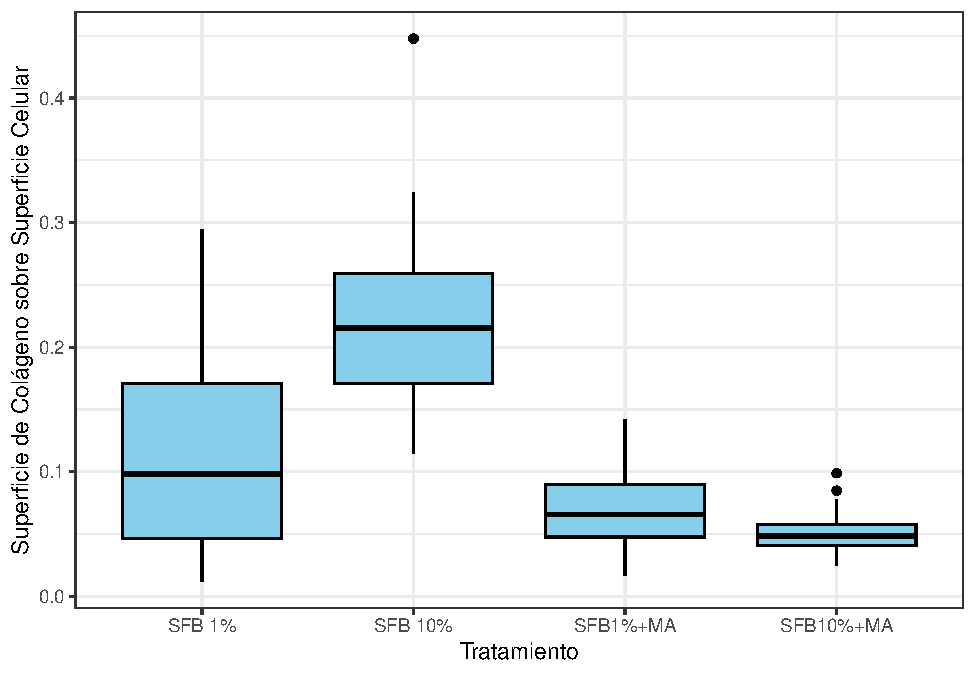
\includegraphics[width=0.55\linewidth,height=0.35\textheight]{Trabajo-Practico-NP_files/figure-latex/unnamed-chunk-4-1} 

}

\caption{Distribución de Superficie de Colágeno sobre Superficie Celular por tratamiento}\label{fig:unnamed-chunk-4}
\end{figure}

El análisis de la distribución de la proporción de superficie celular
ocupada por colágeno muestra que las células tratadas con SFB 10\%
presentan la mediana más alta, seguida por SFB 1\%. En contraste, los
tratamientos combinados con metformina y ácido lipoico (SFB 1\% + MA y
SFB 10\% + MA) presentan medianas más bajas y rangos intercuartílicos
más estrechos, indicando que esta combinación reduce la acumulación de
colágeno en comparación con SFB solo. Además, se observan algunos
valores atípicos en todos los grupos, aunque la tendencia general indica
que la presencia de metformina y ácido lipoico disminuye la proporción
de colágeno.

\newpage

\begin{figure}

{\centering 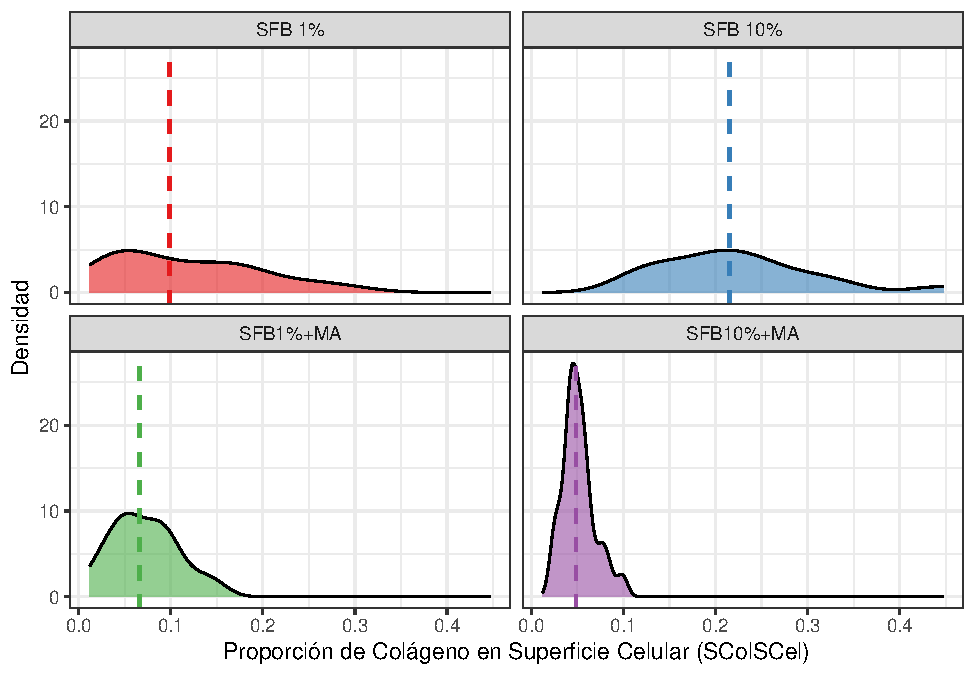
\includegraphics[width=0.55\linewidth,height=0.35\textheight]{Trabajo-Practico-NP_files/figure-latex/fig2-1} 

}

\caption{Distribución de la Proporción de Colágeno por Tratamiento}\label{fig:fig2}
\end{figure}

La Figura 2 sugiere que la aplicación de un test de normalidad no
resulta apropiada, dado que la variable respuesta se presenta como una
proporción. Además, la forma de las distribuciones para cada tratamiento
muestra un claro alejamiento de la normalidad, con asimetrías visibles y
posibles acumulaciones de valores en los extremos.

\section{Análisis estadístico}\label{anuxe1lisis-estaduxedstico}

Para evaluar la adecuación del supuesto de normalidad, se aplicó la
prueba de Lilliefors de manera independiente a cada grupo de
tratamiento. Los resultados mostraron valores de p superiores a 0.05 en
todos los casos, por lo que no se rechazó la hipótesis nula de
normalidad. No obstante, dado que la variable respuesta se expresa como
proporción y que los gráficos de densidad evidencian distribuciones
asimétricas, no resulta adecuado asumir normalidad. Por este motivo, se
optó por emplear métodos no paramétricos para la comparación entre
tratamientos.

Dado lo anterior, se aplicó la prueba no paramétrica de Kruskal--Wallis
para evaluar si existían diferencias en la tendencia central de la
proporción de colágeno en superficie celular (SColSCel) entre las
distintas condiciones de tratamiento. Este enfoque se basa en los rangos
de los datos y no requiere que las observaciones sigan una distribución
normal, resultando apropiado para variables continuas acotadas entre 0 y
1.

Se planteó como hipótesis principal que la distribución de colágeno
(fibrosis) no sería equivalente entre los cuatro tratamientos aplicados
a las Células Estelares Hepáticas (HSC). Se esperaba, en particular, que
la condición de activación fibrogénica (SFB 10\%) generara una mediana
de SColSCel significativamente mayor que el control (SFB 1\%), y que la
combinación con Metformina y Ácido Lipoico (SFB 10\%+MA) mostrara un
efecto reductor sobre la mediana de fibrosis inducida.

Los resultados del test de Kruskal--Wallis indicaron una diferencia
altamente significativa entre los grupos (\(H = 37.936\),
\(p < 0.0001\)). Esto permite rechazar la hipótesis nula de igualdad de
medianas y confirma que las condiciones de cultivo y la inclusión de los
compuestos antifibrogénicos modifican de manera significativa la
tendencia central de la actividad fibrogénica de las HSC.

Para identificar qué tratamientos se diferenciaban específicamente del
control, se realizaron comparaciones múltiples mediante la prueba de
Dunn con ajuste de Holm. El objetivo fue determinar cuáles condiciones
generaban mayor o menor producción de colágeno en promedio.

Los resultados mostraron diferencias estadísticamente significativas
entre el control (SFB 1\%) y los tratamientos SFB 10\% y SFB 10\%+MA (p
\textless{} 0.05), mientras que no se detectaron diferencias
significativas con el tratamiento SFB 1\%+MA. Estos hallazgos sugieren
que las condiciones asociadas a concentraciones más altas de SFB,
especialmente combinadas con Metformina y Ácido Lipoico, inducen un
aumento en la proporción de colágeno en superficie celular en
comparación con el control, mientras que la combinación con SFB 1\%+MA
no genera cambios significativos.

\subsubsection{Análisis de
variabilidad}\label{anuxe1lisis-de-variabilidad}

Para determinar cuáles condiciones generan mayor o menor variabilidad en
la producción de colágeno, se evaluó la dispersión de la proporción de
colágeno en superficie celular (SColSCel) entre los tratamientos. Dado
que la variable respuesta es una proporción y no se cumple el supuesto
de normalidad, se aplicó la prueba de Levene robusta basada en la
mediana (Brown--Forsythe), la cual permite contrastar diferencias en la
variabilidad de manera no paramétrica.

Los resultados de la prueba indicaron que existían diferencias
significativas en la dispersión entre los grupos (\(p < 0.0001\)), lo
que sugiere que existe evidencia muestral suficiente para afirmar que la
variabilidad de SColSCel difiere en al menos uno de los cuatro
tratamientos. Esto permite identificar cuáles condiciones generan una
producción de colágeno más consistente y cuáles presentan mayor
dispersión.

El análisis descriptivo mostró que SFB10\%+MA presentó la menor
variabilidad, indicando una producción de colágeno más consistente,
mientras que SFB 10\% mostró la mayor dispersión, reflejando mayor
heterogeneidad en la respuesta de las células.

\end{document}
